\documentclass[a4paper,12pt,oneside,final]{extbook}

\usepackage[utf8]{inputenc}
\usepackage[T1]{fontenc}

\usepackage{graphicx}
\usepackage{times}
\usepackage[english,swedish]{babel}
\usepackage{tabularx}
\usepackage{geometry}

\geometry{
 margin=20mm
}

\usepackage{fancyhdr}

\usepackage{titling}
\title{Medusa - 3D-rekonstruktion\\Projektrapport, TNM094}
\author{\\Caroline Gard\\Isabell Jansson\\Cecilia Lagerwall\\Johan Reimann\\Erik Sandrén\\Pelle Serander\\Carl Englund}

\frenchspacing
\setlength{\parindent}{0pt}
\parskip 5pt

\usepackage{color}
\definecolor{rltred}{rgb}{.5,0,0}
\definecolor{rltgreen}{rgb}{0,.5,0}
\definecolor{rltblue}{rgb}{0,0,1}

\usepackage[pdftex,
 colorlinks=true,
 urlcolor=rltblue,       % \href{...}{...} external (URL)
 filecolor=rltgreen,     % \href{...} local file
 linkcolor=rltred,       % \ref{...} and \pageref{...}
 citecolor=rltgreen,     % \cite{...}
 pdftitle={},
 pdfauthor={},
 pdfsubject={Projektrapport, TNM094},
 pdfkeywords={},
 pdfpagemode=,
 pdfstartview=FitH,
 bookmarks=true,
 bookmarksopen=false,
 bookmarksnumbered=true
        ]{hyperref}


\begin{document}

\pagestyle{empty}
\thispagestyle{empty}

\frontmatter

\maketitle

\newpage\null\thispagestyle{empty}\newpage
\setcounter{page}{1}
\pagestyle{fancy}

\chapter{Sammanfattning}
Denna rapport behandlar arbetet inom ett projekt i kursen Medietekniskt Kandidatprojekt, TNM094 på Linköpings universitet. Projektets mål var att utveckla ett 3D-scannerbås där en användare har möjlighet att scanna sig själv för att sedan erhålla en solid 3D-modell med färgtextur. Rapporten omfattar huvudsakligen projektets utvecklingsprocess, metodval, verktyg, planering samt resultat.

Projektet har utvecklats agilt med arbetsmetoden \emph{scrum}. Scrum är en flexibel arbetsmetod där utvecklingsteamet arbetar i \emph{sprintintervall}. Varje \emph{sprint} har pågått under två veckor där utvecklingsteamet har arbetat med planerade \emph{tasks} som bygger på kundens krav på systemet. Varje sprint utvärderades vid avslut för att kontinuerligt kunna förbättra arbetsprocessen och lösa eventuella problem.

Scanningen använder sig av tre stycken \emph{Microsoft Kinect-kameror för Xbox 360} och styrs av användaren via en enkel \emph{webbapplikation} som är placerad inuti båset. Webbapplikationen kommunicerar med systemet via en \emph{\textbf{websocketserver}}. Systemet är konstant aktivt och inväntar anrop från webbapplikationen som sker när användaren startar scanningen från användargränssnittet. Den färdiga modellen sparas i en databas. För att komma åt sin modell kan användaren välja att få ett e-postmeddelande innehållande en länk till sin modell. För att säkerställa att användaren endast kommer åt sin egna modell innehåller filnamnet en krypterad sträng.

Utvecklingsteamet har uppfyllt kundens krav för systemet, att skapa en 3D-scanner där användaren erhåller en solid modell av sig själv. Användaren kan även starta systemet via ett enkelt gränssnitt, vilket också var ett krav. Systemet är fortfarande en prototyp och innehåller ett flertal utvecklingsmöjligheter för att betraktas som ett färdigt system.

Arbetsprocessen och verktygen har utvecklingsteamet tagit fram tillsammans efter vad teamet har kompetens för och vad som anses vara mest lämpligt för projektet. Arbetet har lagts upp på det sättet att kundens krav uppfylls under den utsatta tidsperioden.

\tableofcontents

\cleardoublepage
% \phantomsection
\addcontentsline{toc}{chapter}{\listfigurename}
\listoffigures

\cleardoublepage
% \phantomsection
\addcontentsline{toc}{chapter}{\listtablename}
\listoftables

\chapter{Typografiska konventioner}
% Här kan man lägga en lista över typografiska konventioner som används
% i rapporten, om de fungerar bäst i tabell-form. Annars läggs de med
% fördel som avsnitt under ``inledning''.
Nedan listas olika typografiska konventioner, se Tabell \ref{tbl:typokonv}.
\begin{table}[h]
\centering
\caption{Typografiska konventioner}
\label{tbl:typokonv}
\begin{tabular}{| l | l | l |}
\hline
Teckensnitt & Förklaring & Exempel \\ \hline
\textbf{\emph{ABCabc123}} & Tekniska termer, först förekommande  & Projektet utvecklades med en \textbf{\emph{buildserver}}\\
\textbf{ABCabc123} & Programvarubibliotek & För kalibreringen användes \textbf{OpenCV}\\
\emph{ABCabc123} & Engelsk term & Inför varje \emph{sprint} hölls ett möte \\
\hline
\end{tabular}
\end{table}

\mainmatter

\chapter{Inledning}
\label{ch:inledning}
Möjligheten att återskapa objekt från verkliga världen i en virtuell värld har varit ett intresseområde de senaste 30 åren i både underhållningssyfte och för informationsvisualisering\cite{craigroberts}. Det är en process som tidigare krävt komplettering av mänskligt arbete. Med hjälp av ny teknik och mer datorkraft, har denna process kunnat automatiseras till den grad att det som förut skulle kunna ta en vecka nu kan ske på några sekunder. Hårdvaran som har använts har utvecklats och är nu tillgänglig för alla. Detta, i kombination med utvecklingen av \emph{3D-skrivare}, har lett till att intresset för att återskapa objekt blivit ett populärt ämne.

\section{Bakgrund}
I kursen “Medietekniskt kandidatarbete”, TNM094, fick ett utvecklingsteam bestående av sju personer i uppgift att utveckla ett mjukvarusystem för ett 3D-scannerbås för att skapa en modell av användaren i färg. Båset skulle innehålla flera djupkameror för att scanna användaren. Den erhållna punktdatan skulle användas för att skapa en solid tredimensionell modell. Användaren skulle även ha möjlighet att interagera med systemet via ett enkelt gränssnitt. Gränssnittet skulle ha som användningsområde att starta scanning, spara- och kasta modell och göra om scanningsprocessen. En stor del av uppgiften var att arbeta med en agil utvecklingsmetod. Fokus för projektet har legat på att utveckla programvaran till ett fysiskt scanningsbås.

\section{Syfte}
Syftet med rapporten är att framlägga målet med projektet och beskriva arbetsmetoder och verktyg som har behandlats under projektets gång. Syftet är även att ge en tydlig reflektion över metodval för arbetsprocessen och undersöka dessa metoder i verklig miljö. Samtliga medlemmar i projektet ska utveckla en förståelse för teoretiska metoder inom systemutveckling.

\section{Frågeställning}

Nedan listas relevanta frågeställningar berörande projektet:
\begin{itemize}

\item Hur kan ett användande av andra generationens Kinect skapa en 3D-modell med tillräckligt god kvalité, utan komplicerade instruktioner och avancerade inställningar?
\item Vilka krav kan ställas på systemets justerbarhet, för att anpassa systemet efter varje individuell användare, och därmed kunna scanna och rendera en korrekt bild?
\item Vilken eller vilka metoder ska systemet använda sig av för att reducera mängden brus i den insamlade punktdatan?
\item Hur kan utvecklingsteamet, utifrån undersökningar av alternativa sätt för insamling av data, finna den bästa lösningen med avseende på kvalitén hos 3D-modellen och vad är för- respektive nackdelarna med de framtagna lösningarna?

\end{itemize}

\section{Avgränsningar}
Under planeringen inför projektet diskuterades vilka avgränsningar för systemet som skulle göras. En begränsning som bestämdes var att scanningen endast avser en person åt gången och är inte anpassad till flera objekt. Detta på grund av att risken för felaktiga tolkningar under scanningen ökar och därmed kan hål i modellen uppkomma. Detta skulle i sin tur förhöja risken för deformation av den resulterande solida modellen.

En annan avgränsning för systemet var att ingen automatisering av 3D-utskrift för modellen skulle implementeras i systemet. Dagens 3D-skrivare har inte tillräcklig snabb utskrift för en acceptabel väntetid. Däremot ska modellen ha ett format för att användaren själv ska ha möjlighet att skriva ut modellen på egen hand.

\chapter{Relaterat arbete}

\section {Microsoft Kinect för XBox 360}
\label{Kinect}
En \emph{Kinect-kamera} består av en färgkamera, en IR-kamera\footnote{Infraröd-kamera} samt en projektor. Projektorn sänder ut punkter som fångas upp av IR-kameran. Punkterna jämförs sedan med ett referensmönster som erhålls genom att Kinect-kameran skapar ett plan på ett känt avstånd från kamerasensorn. Planet sparas sedan i Kinect-kamerans sensorminne. Genom att jämföra om varje punkt är placerad framför eller bakom planet kan Kinect-kameran avgöra vilka punkter som är synliga eller gömda bakom olika föremål. Denna process utförs automatiskt av Kinecten. För bästa resultat bör det inscannade objektet befinna sig inom ett område av en till tre meter från sensorn, vilket resulterar i mindre brus och bättre upplösning av djupdatan\cite{Kinectsensor}.

\subsection{Kalibrering av färgkamera och IR-kamera hos Kinect}
Eftersom färgkameran och IR-kameran inte har exakt samma position i en Kinect-kamera behöver dessa kameror kalibreras. Utan kalibrering kommer texturen att projiceras på modellen inkorrekt\cite{Kinectsensor}. BBåda kamerorna i Kinecten kalibreras samtidigt genom att använda en bild av ett schackmönster. Båda kamerorna måste sedan extrahera hörnpunkterna i schackmönstret, vilket till exempel kan utföras med hjälp av biblioteket \textbf{OpenCV}. Dessa punkter sparas sedan för att ta fram en \emph{\textbf{translationsmatris}} som beskriver sambandet mellan djupbilden från IR-kameran och bilden från färgkameran. Translationsmatrisen används för att förflytta färgbilden innan den projiceras som textur på objektet. Utöver translationsmatrisen erhålls även koefficienter som beskriver den radiella och tangentiella distorsionen. \cite{detphcomvis}.

\subsection{Positionskalibrering av Kinect-kamerorna}
För att flera kameror skall kunna användas behöver deras position utifrån ett gemensamt origo vara känt. Genom att använda den schackrutiga bilden som ovan för att placera ut origo kan translationsmatrisen och distortionskoefficenterna användas för att skapa en vymatris för kameran. Denna matris kan användas för att transformera bilder och punkter mellan världskoordinater och kamerakoordinater. Positionskalibreringen möjliggör att projiceringen av färg-bilden sker utifrån korrekt vinkel och position på modellen\cite{kinectextrinc}.

\section{Ytrekonstruktion}
För att rekonstruera en 3D-modell utifrån inläst punktdata används flera processer, se Figur \ref{fig:pclflow}. Det första steget innebär att systemet skapar eller läser in punkter, där inläsningen utförs till exempel med en IR-kamera. Sedan reduceras datan för att minska komplexiteten och brus filtreras bort. En yta rekonstrueras utifrån de kvarvarande punkterna. En utförligare förklaring av stegen följer nedan.

\begin{figure}[tb]
  \centering
  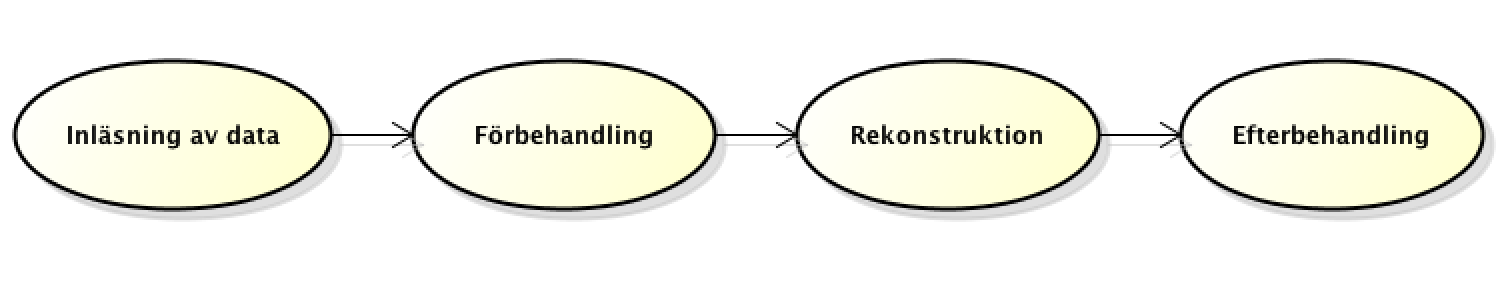
\includegraphics[width=0.9\textwidth]{bilder/pointcloud.png}
  \caption{Processflödet vid ytrekonstruktion}
  \label{fig:pclflow}
\end{figure}

\begin{enumerate}
\item Inläsning av punkdata

Inläsning av de punkter som finns kan ske med till exempel en Kinect-kamera. Processen sker då enligt kapitel \ref{Kinect}.

\item Förbehandling: Reducering av punkdata

Vid inläsning av punktdata via ett flertal Kinect-kameror erhålls punkter i en stor mängd, vilket medför att programmet blir beräkningstungt för datorn. Punkter placerade nära varandra kommer inte att tillföra någon märkbar kvalitetsförändring av modellen. Alla dessa punkter är därmed inte nödvändiga för att erhålla en tillräckligt noggrann tredimensionell modell för ett bra utseende. Reducering av punktdata kommer att underlätta senare beräkningar för datorn. Det finns flera metoder för att utföra reducering av data och det är nödvändigt att avväga vad som viktigast, prestanda eller kvalité.\cite{cluster}

\emph{Voxelgrid-filter} är en metod i biblioteket \textbf{PCL}\footnote{Point Cloud Library} som används för reducering av punktdata. Med denna metod skapas ett tredimensionellt rutnät över den inlästa punktdatan vilket bildar kuber, voxels, utmed ytan där samtliga punkter är uniforma och har samma massa. Punkter som befinner sig i samma voxel används sedan för att uppskatta en ny punkt baserat på tyngdpunkter hos varje punkt i voxeln. Punkterna nedsamplas därmed i samtliga voxels och reduceras efter en approximation beroende på varje punkts placering. Metoden är snabb och ger en relativt hög upplösning av ytan hos modellen. Genom att minska storleken på varje voxel kan även noggrannheten förbättras, men programmet blir dock mer beräkningstungt.
\cite{pclvoxel}


\item Förbehandling: Reducering av brus

Vid scanningen kan det uppstå felaktiga punkter med extremvärden som uppkommer på grund av mätningsfel vid inläsningen. Detta beror på att IR-kameran registrerar felaktig data som exempelvis kan inträffa vid inläsning av partiklar i luften. Felaktiga eller fristående punkter tolkas som brus och måste avlägsnas för att senare kunna skapa en solid modell.

\emph{StatisticalOutlierRemoval filter} är en metod för att hantera brusreducering och är en del av \textbf{PCL}. Brusreduceringen analyserar den statistiska sannolikheten för att en punkts position är relevant i förhållande till sin omgivning. För att identifiera skräppunkter, beräknas det genomsnittliga avståndet för varje punkt till de närmast intilliggande punkterna. Detta genomförs genom att använda både ett globalt medelavstånd samt en lokal standardavvikelse. Det globala medelavståndet har en förbestämd konstant definition medan standardavvikelsen beräknas med radien för varje punkt. De punkter som antar ett större avstånd än beräknat medelvärde kan tolkas som skräppunkter och därmed tas bort från punktdatan\cite{cluster}.

\item Rekonstruktion

För att sammanfoga punkter till en solid modell, används triangulering\cite{pointcloud2surface}. Triangulering innebär att att punkterna omvandlas till vertexpunkter och att kanter och ytor bildar en solid polygonmodell. Det finns flera metoder för rekonstruktion som kan appliceras på punktdatan, dessa med både för- och nackdelar.

Vid rekonstruktionen kan vissa problem uppstå. Metoderna kan till exempel ha svårt att förutse normalriktning om datan har en hög brusnivå. Det kan även finnas områden i datan, exempelvis skuggade områden, som saknar information vilket medför problem hurvida modellen blir solid eller ej. För att hantera problemen finns två kategorier med metoder, globala metoder samt lokala metoder\cite{poisson}.

Globala metoder innebär att hela datamängden behandlas direkt vilket medför att rekonstruktionen för objektet sker på en gång. Globala metoder innehåller ofta implicita funktioner. Funktionerna är växande vilket skapar täta matriser, vilket betyder att de flesta värdena i matrisen är skilda från noll. Dessa matriser har även dåliga villkor som till exempel kan ge felaktiga resultat\cite{poisson}.

Lokala metoder behandlar rekonstruktionen för mindre delar av datan för sig. Hur delarna sedan byggs ihop är en uppskattning av ytan. Lokala metoder ger ett detaltrikare resultat men har en högre känslighet för brus \cite{poisson}.

\emph{Poisson Surface Reconstruction} är en global metod där en ytterlinje skapas baserat på gradienten för en 3D-indicatorfunktion, som fås genom en integralrelation med punkterna. Funktionen är bitvis konstant vilket medför att ytan får obegränsat stora värden. För att undvika det appliceras ett \emph{smoothing filter} på funktionen och gradienter beräknas för den nya funktionen. Användning av Poisson medför därför att följande steg, post-processing, inte behöver appliceras då de redan är inkluderat i metoden\cite{cluster, poisson}.

\item Efterbehandling

Vid inläsning av punktdata via Kinect-kamerorna uppstår det små distansfel mellan vissa av punkterna. Dessa fel orsakar ojämnhet hos modellens yta, vilket måste korrigeras för att modellen ska se tillräckligt bra ut. En ojämn yta kommer att ha normaler med spretiga riktningar, medan en jämnare yta har normaler som förhåller sig bättre till varandra.

En metod som kan användas till att jämna ut ytan, som består av XYZ-koordinater, är marching cubes. Med \emph{marching cubes} sätts de punkter som är placerade längst ut till ett referensplan. Metoden grundar sig i att en vertexpunkt väljs ut och att man därifrån stegar sig fram till de närmaste vertexpunkter med hjälp av \emph{smallest edge detection}\cite{pointcloud2surface}.

\end{enumerate}


\section{Gränssnitt}
\subsection{Websockets}
\emph{Websockets} är en teknik som möjliggör tvåvägskommunikation mellan klient och serverapplikationer. Genom en websocket kan klienten skicka och ta emot information när som helst från en serverapplikation. %[https://www.websocket.org/aboutwebsocket.html 2015-05-11]

\subsection{MongoDB}
\emph{MongoDB} är en \emph{no-sql} dokumentdatabas som använder \emph{BSON}, som är en binär variant av JSON\footnote{JavaScript Object Notation, en dokumenstruktur för javascript objekt}.

\chapter{Arbetssätt}
\section{Arbetsmetoden Scrum}
Projektet har utvecklats agilt med arbetsmetoden \emph{scrum}. En agil arbetsmetod var att föredra eftersom det är en iterativ och flexibel arbetsprocess och scrum är en bra metod för arbete mellan utvecklingsteam och kund. Idén med scrum är att leverera bästa möjliga resultat genom att arbeta kreativt och effektivt för att attackera olika typer av problem. Utvecklingsteamet ska vara av den storlek att arbetet kan utföras effektivt med minsta möjliga antal utvecklare men ändå resultera i ett system av hög kvalité. Samtliga medlemmar i utvecklingsteamet ska arbeta under samma titel, det vill säga en platt hierarki. I och med detta kan varje enskild person i utvecklingsteamet hålla sina arbetsuppgifter rörliga mellan arbetsområdena.

En \emph{produktbacklogg} användes för att lista relevanta \emph{user stories} tillhörande projektet. \emph{Stories} beskriver krav från kund och utvecklingsteam och användes därmed som kravspecifikation för produkten. Projektet delades upp i mindre arbetsperioder, \emph{sprints}, där varje sprint pågick under två veckors tid. Tidpunkten för dessa sprints planerades in i ett \emph{gantt-schema} som utvecklingsteamet använde under projektets gång, se bilaga \ref{app:gantt}. En viktig del för projektteamet var att längden av en sprint var tillräckligt lång för att kunna uppnå ett resultat, utan att sprintens mål blev för komplext. Inför varje sprint  genomfördes en sprint-planering där olika user stories valdes till den kommande sprinten. Varje user story, delades sedan upp i \emph{tasks}, där en task var ett arbetsmål med tidsbegränsningen på högst en dag. För att organisera produktbackloggen och för att planera uppsatta tasks och sprints använde arbetsteamet\emph{Trello}\footnote{www.trello.com}. Alla tasks lades från början i en lista märkt med \emph{“To Do”}. Efter arbetets gång flyttades de sedan till \emph{“Doing”}, \emph{“Under Review”} och \emph{“Done”}, se Figur \ref{fig:trello}. En ofärdig eller ej påbörjad task flyttades till kommande sprint, förutsatt att den ansågs ha tillräckligt hög prioritet för att färdigställas.

Utvecklingsteamet bestod av sammanlagt sju personer men för att effektivisera arbetet delades utvecklingsteamet in i tre mindre ansvarsgrupper; scanning, bildbehandling och gränssnitt.
En beskrivning av ansvarsgruppernas huvudområden följer nedan:

\begin{itemize}
\item \textbf{Scanning}

Gruppen scanning ansvarade för att ta in data från kamerorna, både djup och färg. Gruppen ansvarade även för kalibrering av position och kalibrering av färg- och IR-kamera.


\item \textbf{Bildbehandling}

Gruppen bildbehandling ansvarade för att bygga en solid 3D-modell utifrån den data som kamerorna scannade in.

\item \textbf{Gränssnitt}
Gruppen gränssnitt ansvarade för att bygga ett gränssnitt som användaren kan interagera med, samt att koppla ihop scanningssystemet med gränssnittet.
\end{itemize}

\begin{figure}[htb]
  \centering
  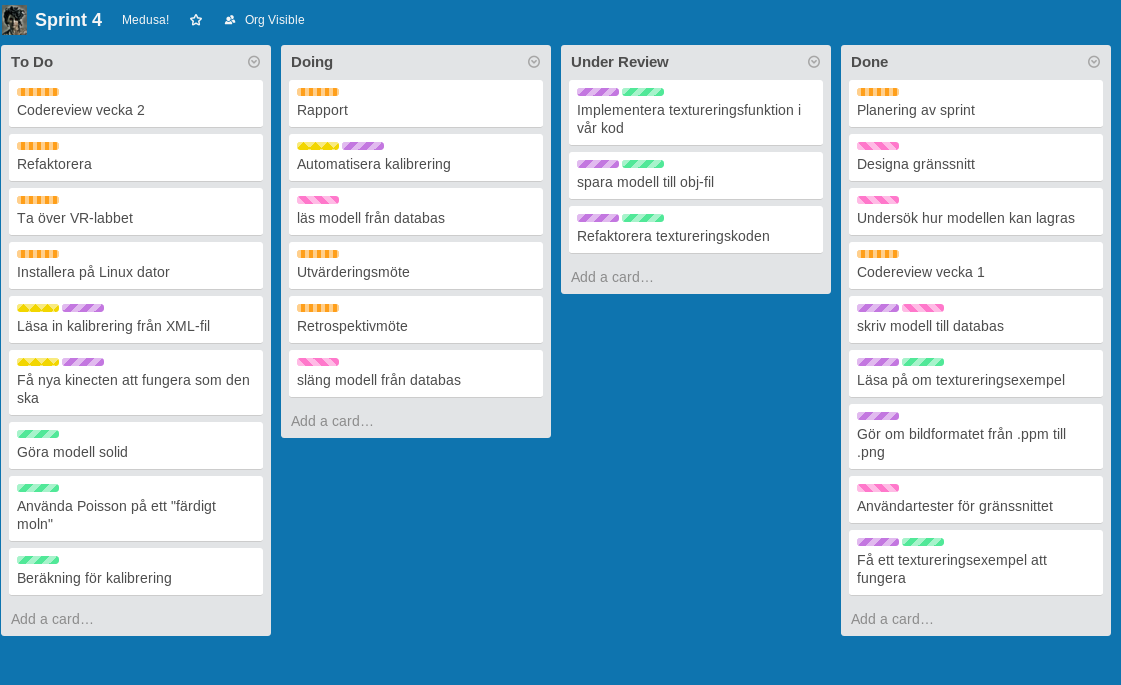
\includegraphics[width=0.9\textwidth]{bilder/trello.png}
  \caption{planering av scrum med hjälp av trello}
  \label{fig:trello}
\end{figure}

Ansvarsgrupperna arbetade parallellt med olika tasks för att effektivt nå målen för projektet. Det var dock viktigt för utvecklingsteamet att vem som helst, oavsett ansvarsområde, skulle kunna sätta sig in andra gruppers arbete.

Utvecklingsteamet tilldelades diverse roller enligt Tabell \ref{tbl:roles} nedan.

\begin{table}[h]
\caption{Roller inom utvecklingsteamet}
\begin{tabular}{|l|l|}
\hline
Produktägare/Kundrelation & \begin{tabular}[c]{@{}l@{}}Produktägarens ansvar var att produktbackloggen hölls uppdaterad\\
                                                       och var prioriterad efter kundens önskemål. Produktbackloggen hade som \\
                                                       krav att vara tydlig och förståelig för hela teamet. Som kundrelation var\\
                                                       ansvaret att kontakta kunden vid behov.\end{tabular} \\ \hline
Scrummästare               & \begin{tabular}[c]{@{}l@{}}Scrummästaren såg till att arbetet följde scrum-metodens krav och \\
                                                        riktlinjer samt styrde de dagliga stående mötena.\end{tabular}\\ \hline
Gruppledare               & \begin{tabular}[c]{@{}l@{}}Gruppledaren hade som uppgift att styra projektet i rätt riktning \\
                                                        och såg till att samtliga gruppmedlemmar följde gruppkontraktet.\end{tabular}\\ \hline
Rapportansvarig           & \begin{tabular}[c]{@{}l@{}}Ansvarade för att rapporten påbörjades i god tid samt att den\\
                                                      höll en hög standard. \end{tabular}\\ \hline
Kodgranskningsansvarig    & Ansvarade för att kodgranskning skedde löpande genom projektet. \\ \hline
Testansvarig              & Ansvarig för att testning av gränssnittet utfördes och utvärderades. \\ \hline
Sekreterare               & \begin{tabular}[c]{@{}l@{}}Sekreteraren ansvarade för att anteckna under varje möte samt att\\
                                                      dokumentera uppkommen information. \end{tabular}\\ \hline
\end{tabular}
\label{tbl:roles}
\end{table}

\subsection{Sprints och möten}
\subsubsection{Stående möte}
Varje morgon inleddes med ett stående möte där hela utvecklingsteamet närvarade. Mötet hölls kort, ungefär tio minuter, och syftade på att sammanfatta gårdagens arbete samt dagens kommande arbete för varje enskild person i utvecklingsteamet. Mötet resulterade i att samtliga gruppmedlemmar fick en inblick i vad som förväntades utföras under dagen och en i de andras arbete. Det medförde även att de olika ansvarsgrupperna hölls uppdaterade om arbetet utanför den egna gruppen.

\subsubsection{Utvärdering av sprint}
Efter varje avslutad sprint hölls ett utvärderingsmöte. Under utvärderingsmötena diskuterade utvecklingsteamet resultatet av sprinten, vad som hunnits med respektive inte hunnits med, vad som kunde bortprioriteras och vad som kunde förbättras inför nästa sprint. Ett exempel på en åtgärd som utfördes efter ett utvärderingsmöte är att de tasks som hade varit för stora behövdes brytas ner till mindre tasks.

\subsubsection{Retrospektivmöte}
Retrospektivmöten skedde i slutet av varje sprint där det togs upp vad som hade gått dåligt respektive bra med arbetssättet under sprinten. Där kom utvecklingsteamet överens om det behövdes ändra någonting till nästkommande sprint och gav förslag på förbättringsmöjligheter som kunde utföras. Ett exempel på vad som förändrades tidigt i projektet var att de stående mötena flyttades bak från 09.00 till 08.30 för att teamet tidigare skulle kunna komma igång med arbetet för dagen och att alla skulle vara uppdaterade med vad andra gjorde.

\subsubsection{Planeringsmöte}
Ett planeringsmöte hölls en gång per sprint och syftade till att välja ut user stories från projektets produktbacklogg inför den kommande sprinten. Varje story delades sedan upp i mindre tasks och utvecklingsteamet diskuterade vad som skulle prioriteras. Utvecklingsteamet valde att planera flera tasks än vad som antogs hinna med och sedan arbeta med de högst prioriterade tasksen. Detta motsäger dock arbetsmetodiken \emph{scrums} grundprinciper, som menar att en sprint ska innehålla de tasks som utvecklingssteamet tror sig hinna med.


\subsubsection{Kodgranskning}
Kodgranskningstillfällen hölls i slutet av varje vecka, alltså två gånger per sprint. Målet med kodgranskningen var att säkerställa att all kod höll en hög standard, var välkommenterad och följde de riktlinjer om kodstandard som utvecklingsteamet hade beslutat om. Det var viktigt för utvecklingsteamet att alla ansvarsgrupperna närvarade oavsett vilken kod som granskades, eftersom koden skulle vara förstålig oavsett vem som skrivit den.

\section{Kravhantering}
Efter första mötet med kunden fick utvecklingsteamet krav som slutprodukten skulle uppnå.
\begin{itemize}
\item Systemet ska vara tillräckligt automatiserat för att en icke insatt användare ska ha möjlighet att använda systemet.
\item Ska kunna se modellen i gränssnittet.
\item Modellen ska vara solid, alltså ett objekt som är slutet.
\item Det ska vara möjligt för användaren att antingen kunna spara eller kasta modellen.
\item Modellen ska vara redo för att kunna skrivas ut på 3D-skrivare.
\item Kunden hade som önskemål att systemet skulle fungera på en dator med operativsystemet Linux.  
\end{itemize}

Ut efter dessa krav gjordes en kravspecifikation, vilket teamets produktbacklogg inkluderar, med krav som går att mäta.

\section{Dokumentation}
\subsection{Textdokument och bildfiler}
Projektet dokumenterades löpande på en gemensam \emph{\textbf{Google Drive}} för att alla i teamet skulle ha tillgång till samtliga dokument. Dokumentationen innefattade anteckningar från utvärderingsmöten, retrospektivmöten, kundmöten etc. På Google Drive sparades även bilder. Mötesanteckningar storterades efter datum samt vilken mötestyp de tillhörde.

\subsection{Koddokumentation}
Alla filer i projektet kommenterades enligt \emph{Doxygens}\footnote{www.doxygen.org} riktlinjer för dokumentation. Dokumentation autogenererades sedan av projektets \textbf{\emph{buildserver}} för enkel åtkomst. Kommentarerna skulle vara tillräckligt tydliga för att en utomstående skulle kunna förstå syftet med bland annat funktioner. Alla funktioner kommenterades men även kommentarer för enstaka rader utfördes i funktionerna för att förtydliga användandet och syftet.

\section{Versionshantering}
\emph{Git} användes för versionshantering under projektet. För att dela koden användes \emph{Github} med välkommenterade \emph{commits} om vilka ändringar som utförts vid varje \emph{push}.

För att enkelt separera olika delar i projektet använde utvecklingsteamet olika grenar. Det fanns tre olika huvudgrenar förutom \emph{develop} och \emph{master}. Dessa var bildbehandling, scanning och DART-utveckling. DART är ett programmeringsspråk som är \textbf{open-source}, skalbart och anpassat för web-applikationer. Förutom dessa grenar skapades även separata grenar av alla utvecklare för att arbeta på mindre funktionaliteter. Dessa kunde sedan implementeras in i huvudgrenarna.

\section{Testning}
Testningen som har genomförts innefattar användartester på gränssnittet samt kodgranskningar för att säkerställa att en god kvalité hölls och koden följde de bestämda riktlinjerna. Kodgranskningarna underlättade även för olika ansvarsgrupperna att förstå varandras kod.

\emph{Jenkins}\footnote{www.jenkins-ci.org} har använts för \emph{continuous integration} och har försökt bygga innehållet vid varje \emph{push} till \emph{develop}-, eller \emph{master}-grenen. Om kompileringen misslyckades skickas ett felmeddelande till den ansvariga personen laddat upp filen på den påverkade grenen. Jenkins användes även för att autogenerera dokumentationen till projektet med hjälp av Doxygen.

För att säkerställa att gränssnittet var enkelt och intuitivt genomfördes användartester. Innan testet inleddes informerades testpersonerna med samma information som de hade fått om de hade varit på plats i båset. De blev alltså informarade om att de befann sig i ett 3D-scannerbås och att de hade en surfplatta framför sig. Testpersonerna fick sedan själva komma fram till vad som behövde göras för att utföra scanningen. Under tiden ombads de att beskriva sina tankar om både funktionaliteten och det grafiska. Även utvalda frågor ställdes till deltagarna. Totalt utfördes fem användartester på fem olika personer, vilket ansågs som tillräckligt. Gränssnittet uppdaterades sedan efter testpersonernas anmärkningar.

\chapter{Redogörelse för arbetet}
\section{Systemarkitektur}
Vid projektets start utfördes en enkel systemarkitektur för att säkerställa att utvecklingsteamet strävade mot ett gemensamt mål, samt för att på en abstrakt nivå veta hur systemet skulle se ut, se Figur \ref{fig:oldArch}.

\begin{figure}[ht]
  \centering
  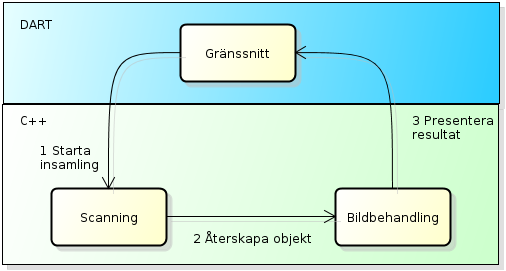
\includegraphics[width=.9\textwidth]{bilder/oldarch.png}
  \caption{Ursprungliga systemarkitekturen}
  \label{fig:oldArch}
\end{figure}

Ovanstående systemarkitektur användes sedan som grund för projektet och utvecklades under processen och blev allt mer detaljerad, se Figur \ref{fig:newArch}.

\begin{figure}[ht]
  \centering
  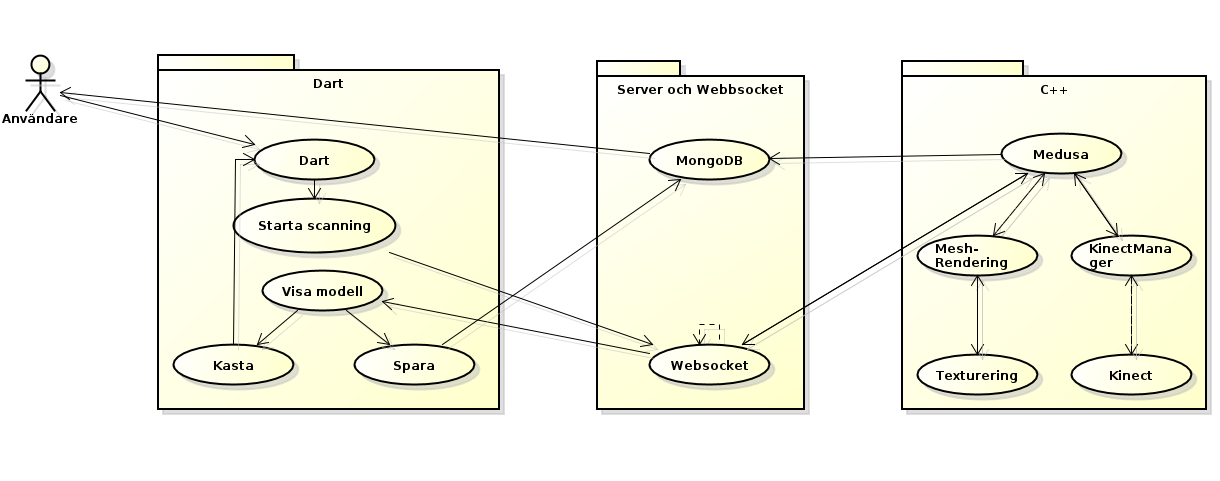
\includegraphics[width=0.9\textwidth]{bilder/newarch.png}
  \caption{Den nya och utvecklade systemarkitekturen}
  \label{fig:newArch}
\end{figure}

\section{Systemets delar}
\subsection{Scanning}
\subsubsection{Hårdvara}
För att genomföra scanningen användes Microsofts Kinect-kameror för Xbox 360. En viktig fråga för utvecklingsteamet var hur insamlingen av data skulle hanteras där två möjliga alternativ fanns tillgängliga. Antingen kan kamerorna vara utplacerade på fasta bestämda platser. Metoden medför att flera kameror måste användas för en total täckning av det scannade objektet. Vid undersökning av att scanna en kropp visades att tre kameror, jämt utplacerade, var tillräckligt antal för denna metod. Det andra alternativet var att använda en kamera som sedan roterar runt objektet. Metoden avvisades då den ansågs svår att genomföra rent praktiskt. Eftersom det huvudsakliga målet inte var att skapa det fysiska systemet, valdes ett system med kameror med fasta positioner.

\subsubsection{Kalibrering av kamerornas position}
För att underlätta uppsättningen av det fysiska båset för kunden gjordes en kalibreringsfunktion av kamerornas position. Målet med kalibreringen var att kamerorna ska veta sin position i förhållande till ett gemensamt origo.

Vid en kalibrering måste först Kinect-kamerorna kalibreras enskilt för att ta reda på deras interna distortionskoefficienter och kameramatris. Detta sker genom att låta alla kameror ta bilder kontinuerligt och försöka hitta schackbrädet,ref teori, i tio stycken individuella bilder. Utifrån dessa tio bilder kan koefficienter och en kameramatris tas fram för att sedan kalibrera Kinect-kamerornas position. En funktion för att sedan få alla Kinect-kameror att ta en bild samtidigt på schackbrödet skapades. Dessa bilder kunde användas för att skapa ett gemensamt origio för alla Kinect-kameror\cite{kinectextrinc}.

\subsection{Bildbehandling}
För bearbetning av djupdata användes \textbf{PCL}. \textbf{PCL} är en samling av moderna algoritmer och metoder för att hantera 3D-data för både företag och privatpersoner. Bibliotekets uppbyggnad är modulbaserat vilket innebär att det är ett relativt enkelt att hantera metoder för önskad funktionalitet\cite{pcl}.

\subsubsection{Scanningsprocessen}
För att minska risken för förbisedda punkter och få en tillräckligt stor täckning av objektet användes tre stycken Kinect-kameror, positionerade enligt Figur \ref{fig:kinect}. Punkterna hos det scannade objektet registrerades med Kinect-kamerornas IR-kameror, enligt kapitel \ref{Kinect}. Bruspunkter i punktdatan rensades bort med metoden \textbf{\emph{StatisticalOutlierRemoval filter}}, en metod i \textbf{PCL}.

\begin{figure}[tb]
  \centering
  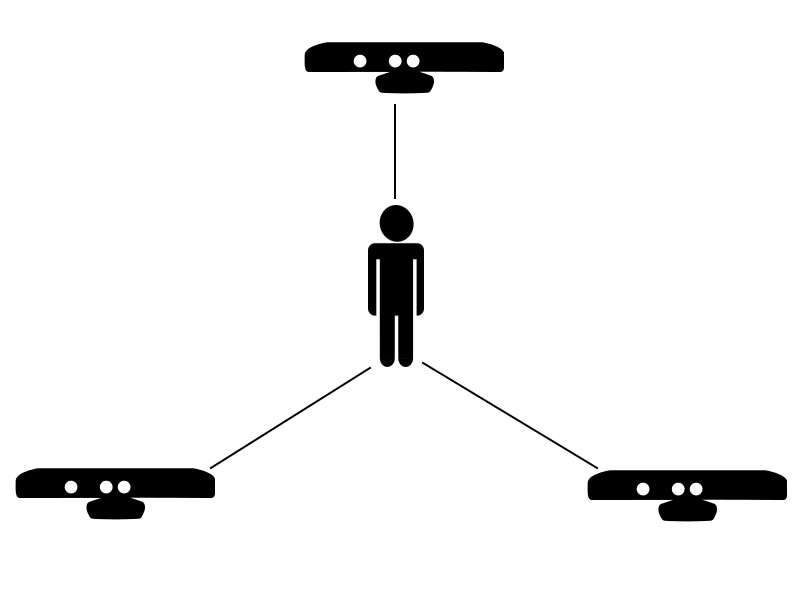
\includegraphics[width=0.9\textwidth]{bilder/setup.png}
  \caption{Kinect-kamerornas position.}
  \label{fig:kinect}
\end{figure}


En nedsampling av punktdatan kunde sedan utföras genom att applicering av voxelgrid filter, även denna en metod i \textbf{PCL}, och en stor del av punktdatan kunde reduceras. Denna metod verkställde en reducering på ungefär 90 procent av punktdatan, detta utan någon märkbar skillnad av kvalité hos den resulterande modellen. Däremot gav metoden ingen betydande skillnad i beräkningshastigheten hos systemet. Poissons metod för ytrekonstruktion applicerades sedan med hjälp av \textbf{PCL} på punkdatan för att skapa en solid modell\cite{cluster}.

\subsubsection{Texturering}
Till textureringen av 3D-modellen användes färgkamerorna för att ta bilder som projicerades på modellen. Eftersom varje Kinect-kamera ger en bild kommer flera texturer att projiceras på objektet, men från olika vinklar. När kamerornas position kalibreras erhålls en matris som beskriver hur varje färgbild behöver transformeras för att projiceras på modellen på en korrekt plats. Texturen projiceras på modellen med hjälp av \textbf{PCL}.

\subsection{Gränssnitt}
Gränssnittet utvecklades som en webbapplikation med målet att därifrån kunna styra scanningsystemet. Det var viktigt att gränssnittet var enkelt och intuitivt att använda och användartester har därför genomförst, se stycke 3.5. Webbapplikationen visas på en touchskärm där användaren enkelt startar scannern. För att gränssnittet ska kunna kommunicera med scanningsystemet har websockets implementeras på klientsidan med hjälp av \textbf{DART}.

\subsection{Websockets}
Websockets användes för att kommunicera mellan webbapplikation och den stationära datorn där själva programmet körs, för detta användes biblioteket \textbf{libwebsockets} på serversidan. Detta bibliotek valdes för att det var enkelt och avskalat vilket passade bra då det bara behövdes skickas små korta meddelanden. När ett meddelande skickas till servern tas detta emot och servern distribuerar ut uppgifter till de olika delmodulerna i systemet.

\subsection{MongoDB}
För att lagra filerna används MongoDB, vilket möjliggör lagring av \emph{obj-filerna} direkt i databasen med ett \emph{MD5}-krypterat datum samt ett nyckelord som id. Nyckeln kan sedan skickas till användaren via epost om användaren bestämmer sig för att spara modellen samt användas för att radera modellen i annat fall. Klassen \emph{GridFS} användes för att undvika problem med filernas storlek. Stora filer delas då upp i flera delar i databasen.


\chapter{Resultat}
\section{Scanning}
Projektarbetet resulterade i ett system som utför en scanning med ett flertal sammankopplade Kinect-kameror. Hårdvarans prestanda avgör hur många Kinect-kameror som kan användas samtidigt. Dock är minsta möjliga antal kameror för en total scanning tre stycken om resultatet ska ha full täckning. Systemet är utformat för att sättas upp i ett bås med en skärm på insidan som via ett gränssnitt går att interagera med.
\section{Gränssnitt}
Bilden nedan representerar gränssnittets utseende och vad som händer när användaren interagerar med de olika knappalternativen. Användaren möts först av sidan som visas på skärmen högst upp till vänster. Där finns det två alternativ en knapp med texten “Info” som leder till skärmen högst upp till vänster. Där får användaren information om projektet och om systemet. Andra knappen med texten “START” på leder vidare i scanninngsprocessen. En kort information om vad användaren ska göra för att starta scanningen och en tillhörande knapp under informationen som leder till sidan längst ner till höger. Den sidan visar en nedräkning på när scanningen startas och användaren hinner ställa sig i den position den vill bli scannad i. När nedräkningen når noll kommer användaren vidare till nästa sida som visar en laddningssymbol på hur långt scanningen har kommit. När den är fylld kommer användaren till sista sidan och 3D-modellen visas och får då tre alternativ.

\begin{figure}[h]
  \centering
  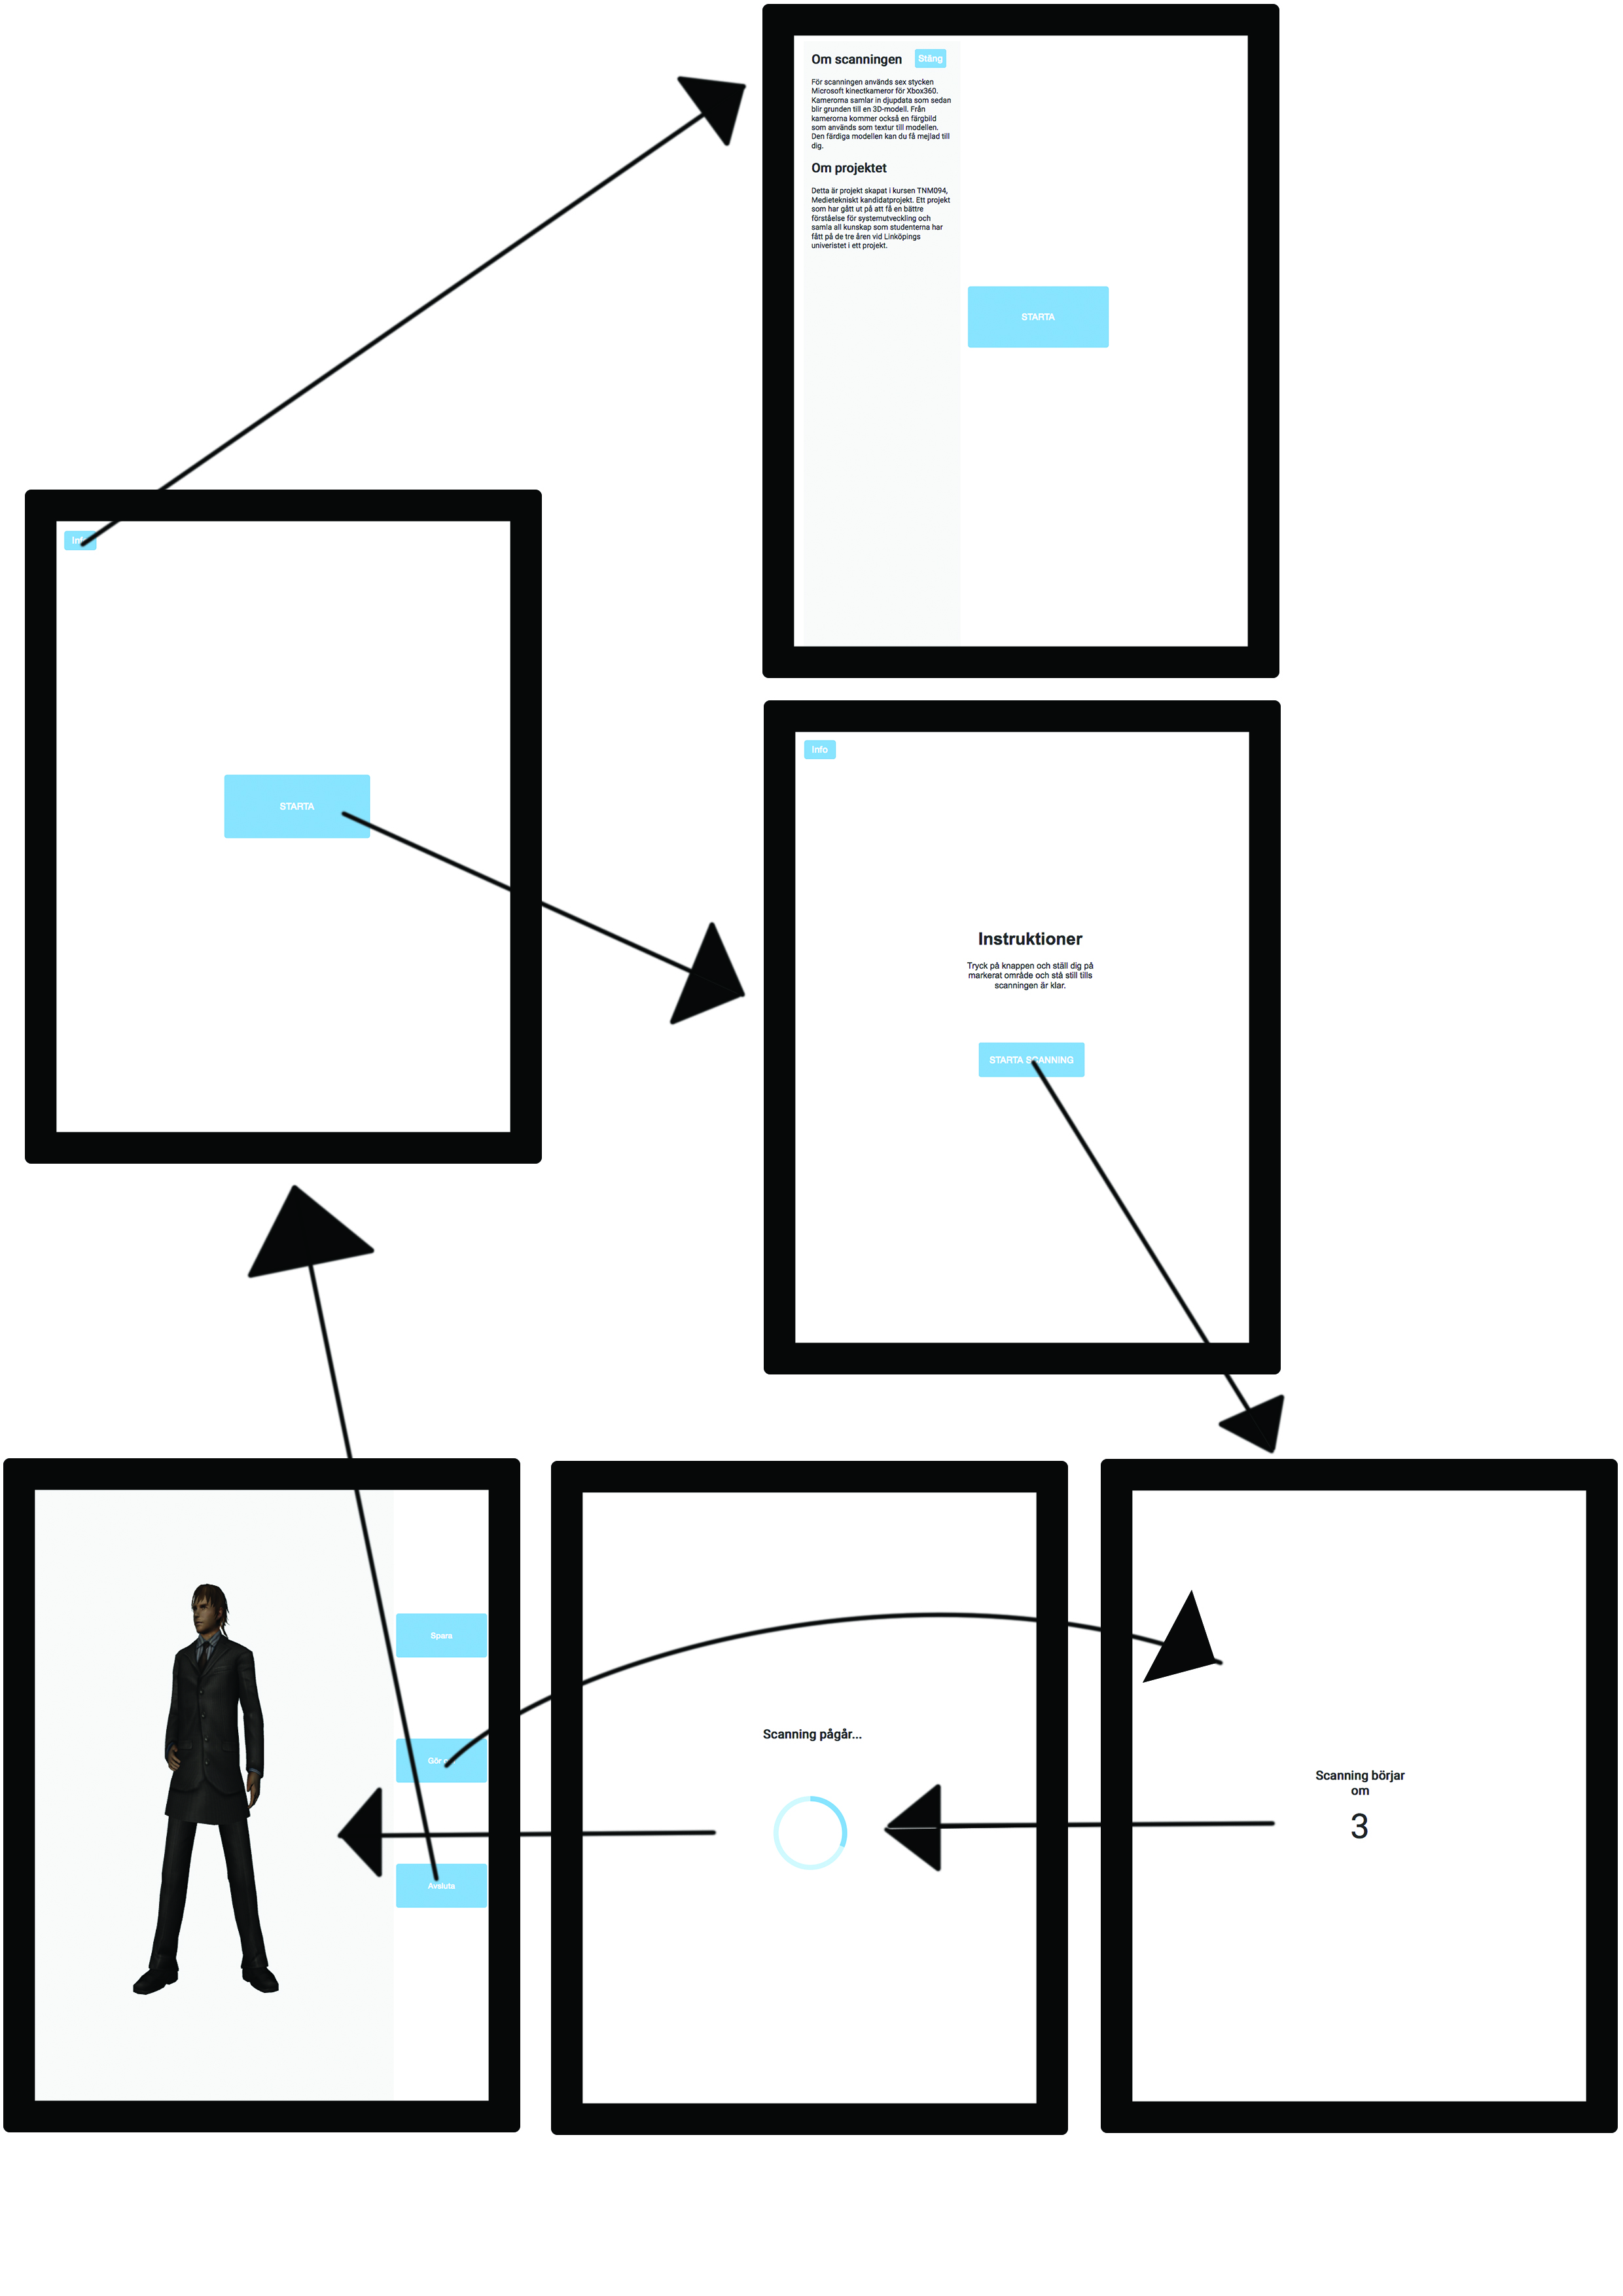
\includegraphics[width=0.85\textwidth]{bilder/granssnitt.jpg}
  \caption{Gränssnittet när modellen presenteras för användaren}
  \label{fig:gui}
\end{figure}

Användaren kan välja mellan att spara, gör om och avsluta systemet. Varje alternativ visar ett pop-up fönster enligt figuren ovan. Väljer användaren att spara kommer det upp ett fönster där en e-postadress kan skrivas in. Här valideras e-postadressen till den grad att användaren behöver skriva in rätt format på adressen, alltså kontrolleras inte att adressen finns. Stämmer inte formatet på adressen måste användaren skriva om adressen igen. Stämmer adressen får användaren en återkoppling om att modellen är sparad och skickad till den angivna adressen. Användaren kommer då tillbaka till sidan där modellen visas men det är nu inte längre möjligt att spara om modellen på nytt. Väljer användaren att göra om modellen kommer det upp ett fönster som frågar om användaren är säker på att användaren vill göra om modellen och talar om att nuvarande modell kommer att kastas, detta visas i figuren ovan på den mellersta skärmen. Nu hamnar användaren tillbaka till det steget där användaren ska ställa sig i position för scanningen. Sista alternativet, “Avsluta”, fungerar som “Gör om” men användaren kommer nu komma tillbaka till första skärmen.

\begin{figure}[h]
  \centering
  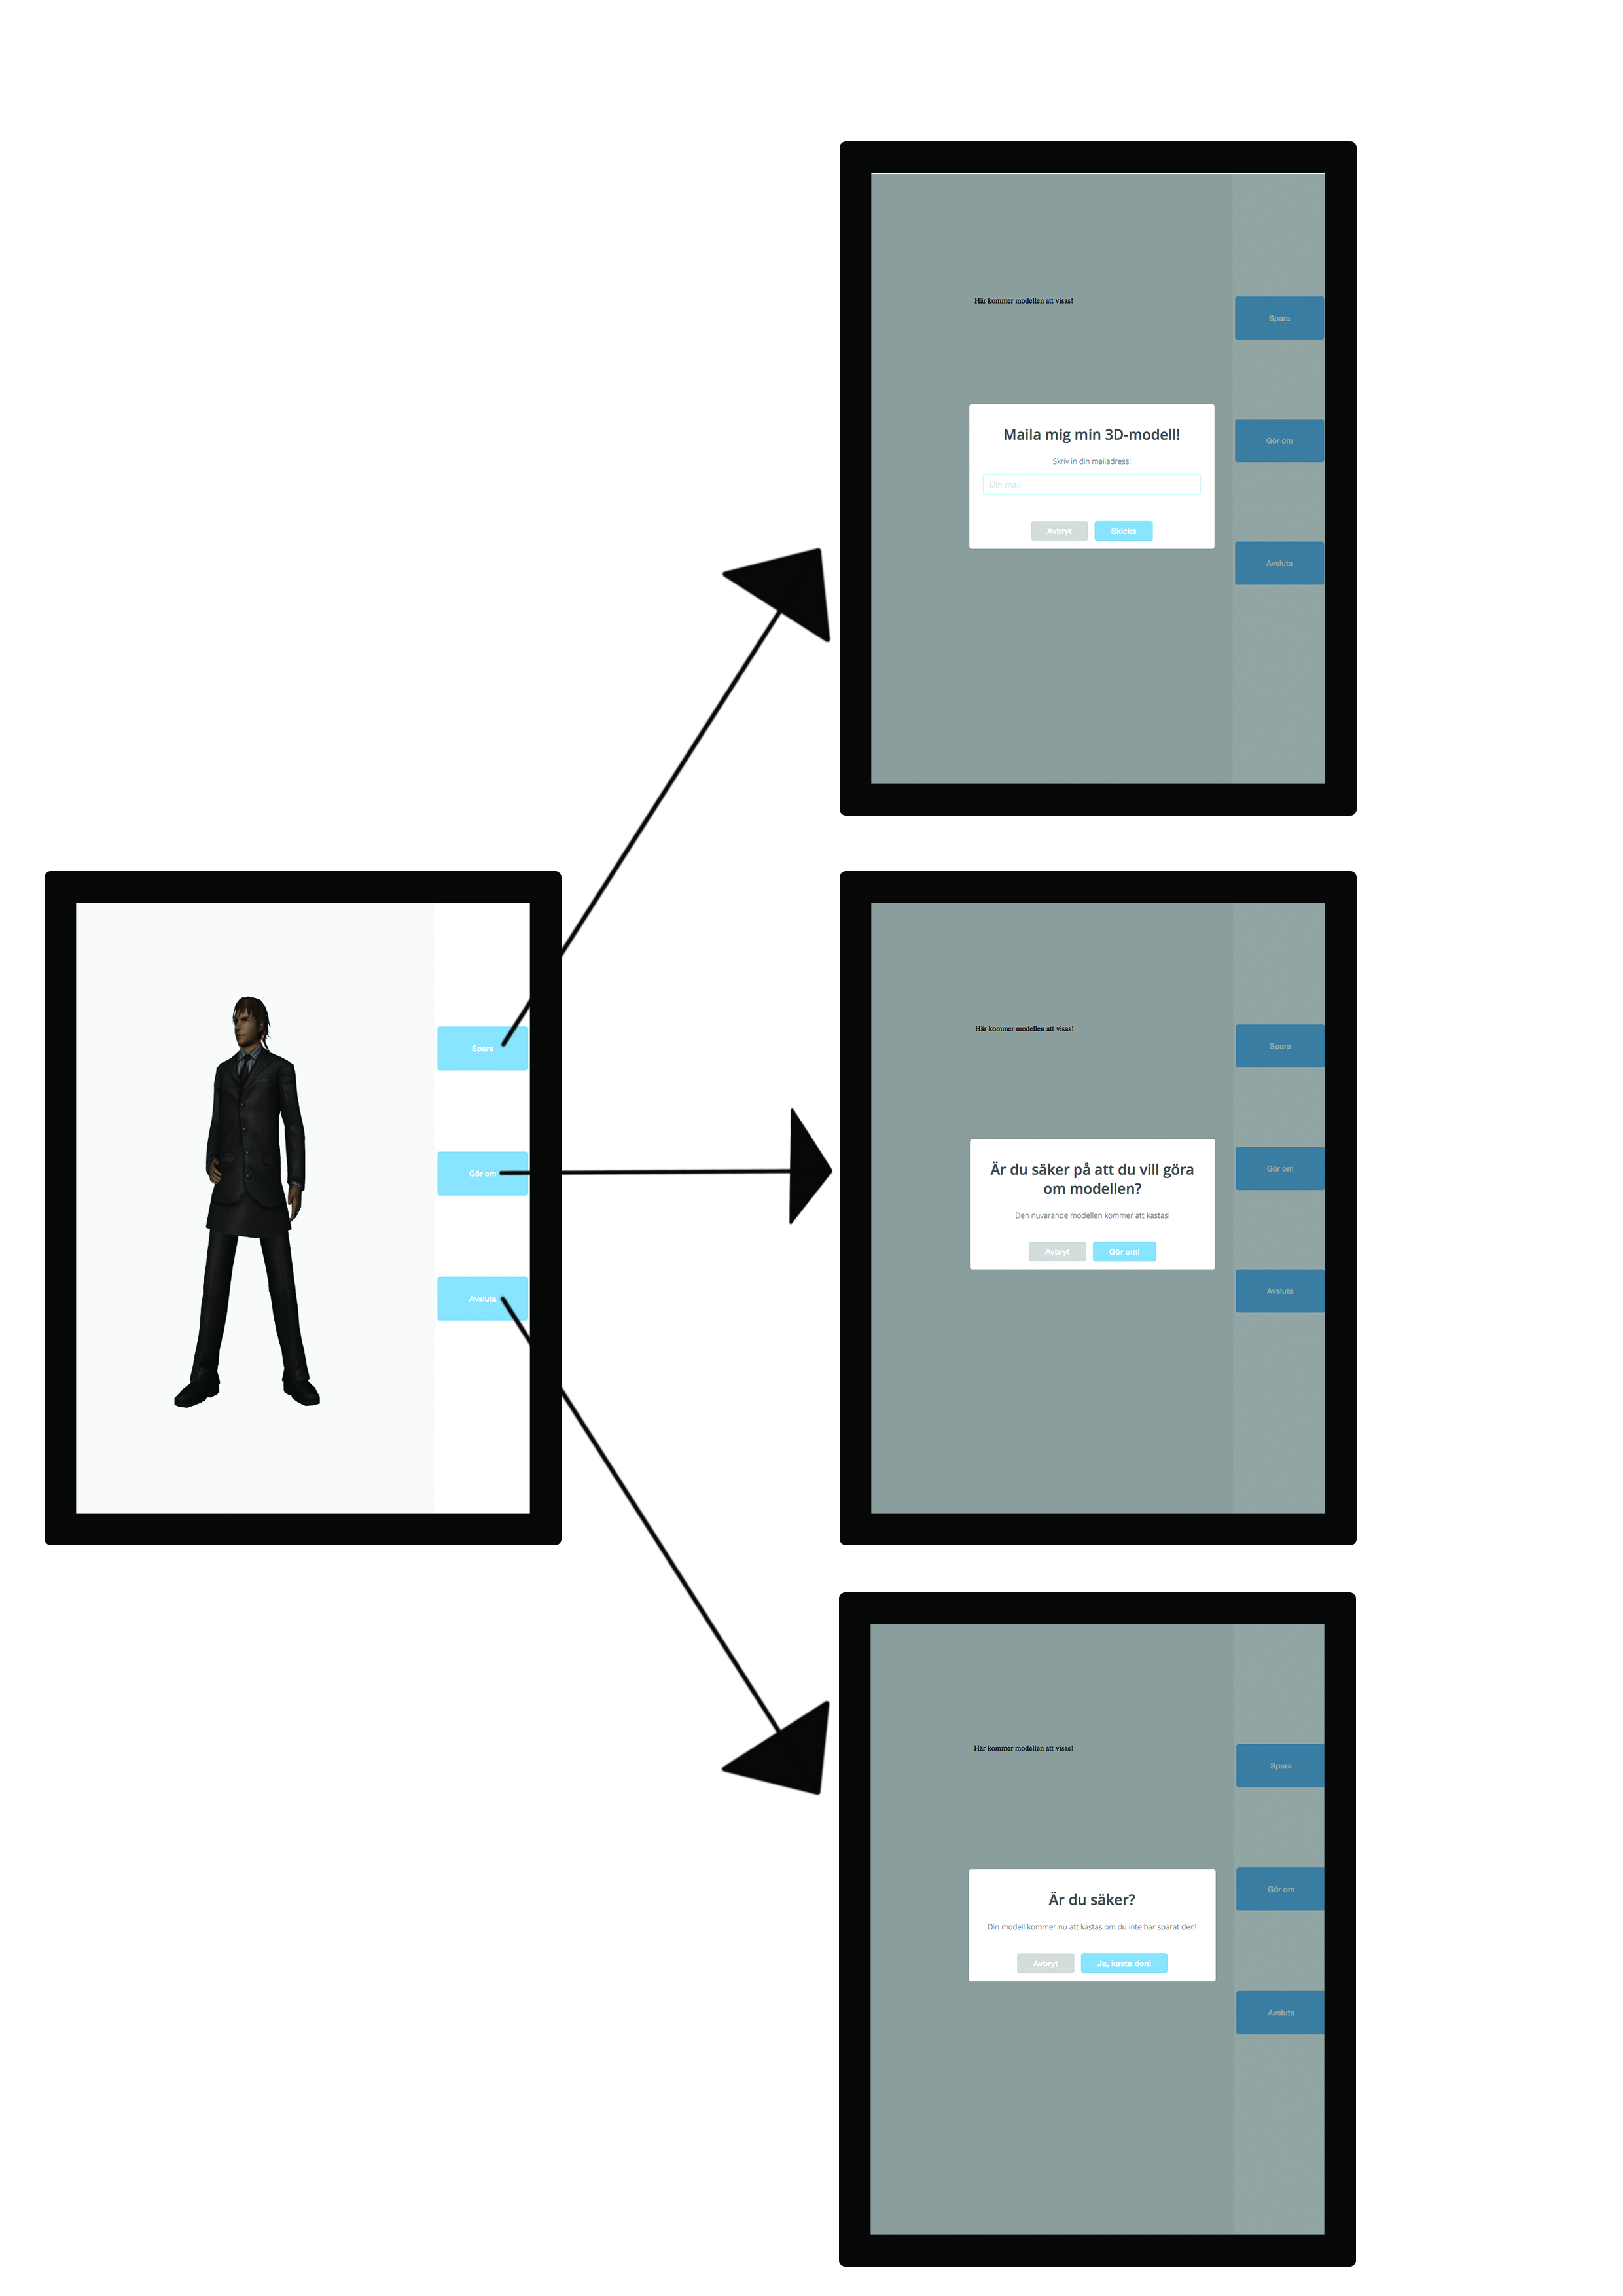
\includegraphics[width=0.85\textwidth]{bilder/save_doover.jpg}
  \caption{Gränssnittet när modellen presenteras för användaren}
  \label{fig:gui}
\end{figure}

\newpage
\section{Bildbehandling}
Enligt teorin kan en IR-kamera användas till att samla in punkter som sedan kan användas till att skapa en solid 3D-modell. Ett \emph\textbf{{voxelgrid filter} kunde användas för att sampla ner insamlad data till en mer lämplig mängd. Vidare kunde metoden \emph\textbf{{StatisticalOutlierRemoval filter} användas för att reducera onödigt brus. Som rekonstruktionsmodell användes \textbf{PCL}s klass Poisson för att applicera en rekonstruktionsmodell.

I bildserien nedan, se Figur \ref{fig:scans}, visar en stegvis behandling av data för scanning utförd av en Kinect-kamera. Scanningen är utförd med endast en kamera vilket resulterar i ett oönskat resultat efter Poissons metod för ytrekonstruktion. Metoden vet inte hur objektet ska byggas ihop då täckning saknas.


\begin{figure}
\centering
\mbox{\subfigure{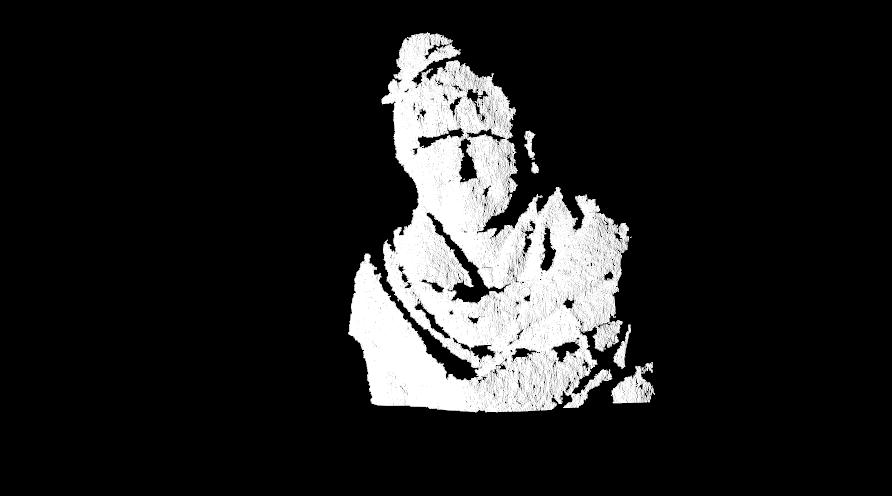
\includegraphics[width=.5\textwidth]{bilder/bilddata1.png}}\quad
\subfigure{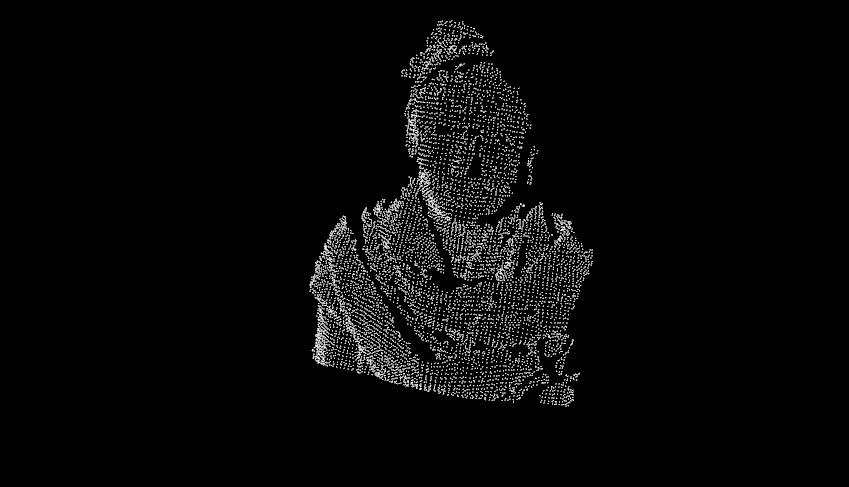
\includegraphics[width=.5\textwidth]{bilder/bilddata2.png} }}
\mbox{\subfigure{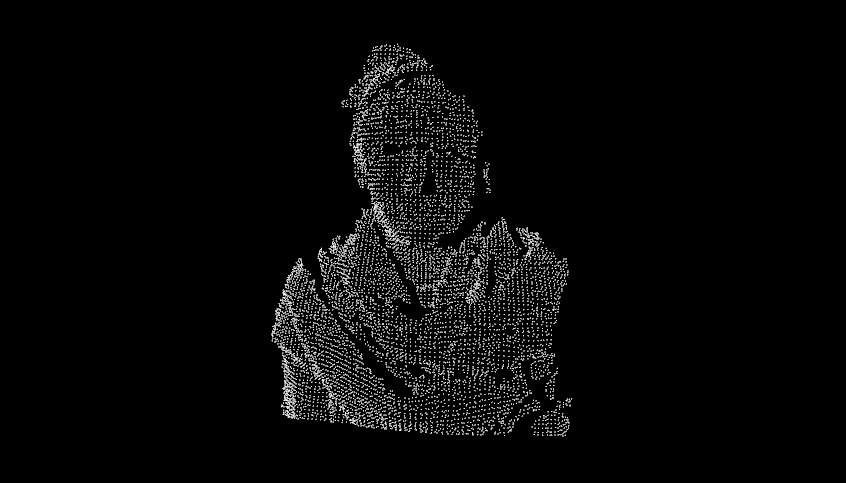
\includegraphics[width=.5\textwidth]{bilder/bilddata3.png}}\quad
\subfigure{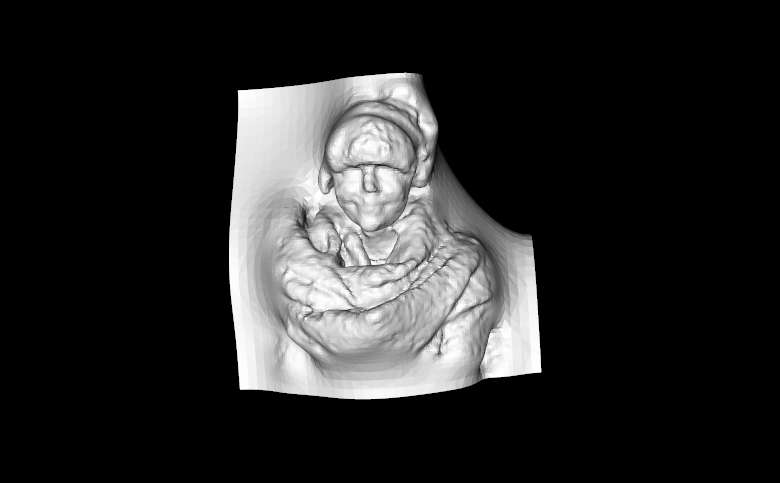
\includegraphics[width=.5\textwidth]{bilder/bilddata4.png} }}
\caption[Bilder från ytrekonstruktion]{(A) Bild på rå punktdata. (B) Reducering av punktdata. (C) Reducering av brus. (D) Yta med Poissons metod för ytrekonstruktion} \label{fig:scans}
\end{figure}

\chapter{Analys och diskussion}
\section{Metod}
De valda metoderna i projektarbetet är bestämda efter de kompetenser som teamet besitter och resurser som ledningen har kunnat bistå med. Det finns delar som teamet hade utfört annorlunda om projektet skulle genomföras en gång till eller om förhållanden hade varit annorlunda, som till exempel att teamet hade haft en längre tidsperiod på sig. Metodernas för- och nackdelar kommer i det här stycket att diskuteras och analyseras.

\subsection{Scanningsprocessen}

Teamet valde att scanna med Microsofts Kinect-kameror för Xbox 360 som är utvecklat och anpassat framförallt för Windows. Eftersom teamet valde att utveckla ett system som passar till Linux, OS X och till Windows valdes biblioteket \textbf{libfreenect}. Biblioteket är öppen källkod som har utvecklats av personer med eget intresse för att skapa system till Kinect-kameror. Alternativet hade varit att enbart utveckla till Windows och då kunnat använda Kinect-kamerornas tillhörande bibliotek \textbf{Kinect for Windows SDK} som har finansiellt stöd från Microsoft och då större möjligheter till att utvecklas. Med \textbf{Kinect for Windows SDK} finns det större möjligheter och det är lättare att utveckla systemet då biblioteket har fler färdiga funktioner än \textbf{libfreenect}.

För projektet valdes det att använda tre Kinect-kameror som tillsammans scannar in en människa. För att inte missa viktig information om punktdatan behövs det minst tre kameror, detta gäller om Kinect-kamerorna är statiskt placerade. Fördelen med att använda minsta möjliga antal Kinect-kameror är att detta minskar mängden data som tas in i systemet, utan att påverka kvalitén för den resulterande 3D-modellen. Detta bidrar till mindre beräkningar för datorn. Nackdelen är att kamerorna är placerade runt objektet och det är därför möjligt att missa information om vissa delar är täckta av andra och missar även informationen som är på objektet, till exempel huvudets topp. Detta gör att systemet gissar hur objektet ser ut bakom dolda delar. En lösning hade varit att ha fler kameror för att ta in mer information om objektet. Risken blir då att systemet blir trögt och i värsta fall inte uppfyller kravet att användaren ska uppleva systemet tillräckligt snabbt. En annan lösning på problemet, som tidigare har nämnts i rapporten, är att ha en rörlig kamera. Detta var inte praktiskt möjligt med de resurser som teamet hade. En rörlig kamera som snurrar kräver en mer komplicerad anordning och eftersom teamet inte hade som krav att faktiskt bygga det fysiska båset blev det en ytterligare faktor till att inte ha en rörlig kamera.

\subsubsection{Kalibrering av djup- och färgkamera}
Kalibering av djup- och färgkamera undersöktes, men prioriterades senare bort. Resultatet skulle hypotetisk bli ännu bättre med en kalibrering, men ansågs ändå tillräckligt bra för att lämnas till senare arbete.


\subsection{Ytrekonstruktion}
Reduceringen av data som användes av systemet är effektiv och tillräckligt snabb för att köras inom en rimlig tid. Användaren behöver endast vänta en kortare stund innan processen är klar. Nedsamplingsmetoden tar bort cirka 90 procent av punkterna i scenen. Det finns flera olika metoder för själva ytrekonstruktionen. Metoden som valdes, Poisson, gav en bra blandning av jämna och solida ytor. Andra metoder som testades var \emph{greedyprojectiontriangulation}, \emph{marching cubes}, \emph{marching cubes hoppe}  och \emph{moving least squares}. Ingen av dessa metoder skapade en solid yta, vilket var ett av kraven på projeket, och därför valdes de bort.


\subsection{Gränssnittet}
Målet med gränssnittet var att göra det lätt för användaren att hantera systemet utan direkta instruktioner och att det skulle vara snabbt och enkelt att använda. Detta eftersom systemet har ett större användningsområde vid allmänna platser snarare än för privat bruk. Gränssnittet visas på en touchskärm eftersom detta är enkelt och snabbt att interagera med och förstå.

Gränssnittet utvecklades som en webbapplikation då utvecklingsteamet hade mer erfarenhet inom webbutveckling jämfört med gränssnittsutveckling inom exempelvis C++. Det var även enklare att få igång gränssnittet och bedriva användartester på en touchskärm.


\section{Resultat}
Resultatet förhåller sig bra till vad som kunde förväntas. Det kan dock variera beroende på hur kamerorna är placerade samt i vilken position användaren står i. Det kan uppstå situationer där vissa ytor inte uppfattas av IR-kameran vilket gör att rekonstruktionsmodellen uppskattar hur ytan borde byggas ihop för att skapa en solid modell.

Eftersom resultatet har en estetisk synvinkel finns vissa svårigheter med att mäta hur bra resultatet är. Utvecklingsteamets mål var att att modellen skulle vara solid, vilket har uppnåtts. En färdig 3D-modell är lik den scannade människan och kan därför ses som ett bra resultat.

\section{Arbetet i ett vidare sammanhang}
I ett vidare sammanhang skulle en 3D-skrivare möjligen kunna kopplas direkt till systemet. Med detta skulle användaren direkt kunna få en fysisk modell efter scanningprocessen istället för en digital 3D-modell via e-post. Om modellen skulle skrivas ut behöver det vara inom en rimlig tid, något som inte finns tillgängligt idag med dagens 3D-skrivarteknik. Skrivaren skulle även behöva skriva ut modellen med tilhörande textur för bästa resultat.

\subsection{Samhälleliga aspekter}
Vill samhället att en person ska ha möjlighet att skapa en ny identitet i ett spel som sig själv? Detta är en fråga som kanske inte har ett rätt svar. Om den här tekniken överfördes på spel, skulle det kunna tänkas att personer som redan lever sina liv på Internet blir ännu mer isolerade genom att faktiskt överföras till en fysisk kropp. Detta skulle i sin tur generera en större grad av passivitet från denna grupp av människor.

Hur ska sparad data hanteras? Om produkten blir kommersiell på exempelvis Microsoft och det där börjas scannas människor, vilka lagar gäller då? Skulle företaget exempelvis kunna använda modellerna utan personens vetskap genom att personerna skulle godkänna en policy.

\section {Problem som har uppstått under projektet}
Utvecklingsteamet fick sent i projektet tillgång till en Kinect för Xbox One. Det bestämdes dock att fortsätta fokusera på de första kamerorna eftersom all kod hade skrivits för dessa och att göra om kodbasen för den nya kameran skulle ta onödig tid. Prestandaskillnaden mellan de båda kamerorna är inte märkbar för projektets användningsområde.

Någonting som har varit tidskrävande var att länka alla bibliotek på gruppens datorer. Då det har utvecklats på olika plattformar har installationsstegen för projektet varit olika. Detta har lett till att mycket tid har lagts på att konfigurera och förbereda för att överhuvudtaget kunna utveckla.

Utvecklingsteamet hade från början planerat att använda Googletest samt DARTs inbyggda testsystem. Efter hand upptäcktes dock att den typen av test inte var lämpade för projektet. En stor del av projektet handlade om att få modellen tillräckligt estetiskt tilltalande vilket inte är mätbart med dessa testmetoder.

\chapter{Slutsatser}
Rapporten syftade till att framlägga målet med projektet samt beskriva arbetsmetoder och verktyg som har använts under projektets gång. Rapporten har även reflekterat över projektets metodval och gett en förståelse för hur valda systemutvecklingsmetoder har fungerat i en verklig miljö.

\section{Svar på frågeställningar}
\begin{itemize}
\item \textbf{Hur kan ett användande av andra generations Kinect skapa en 3D-modell med tillräckligt god kvalité, utan komplicerade instruktioner och avancerade inställningar?}

Utvecklingsteamet beslutade att använda första generationens Kinect då det var det som fanns tillgängligt från början. Det ansågs sedan inte tillräckligt prioriterat att byta till andra generationens Kinect eftersom prestandaskillnaden mellan dessa två kameror inte motiverade de ändringarna som skulle behöva göras i kodbasen. Kinect-kamerorna används för att läsa in punktdata med hjälp av den inbyggda IR-kameran. Punktdatan kan sedan användas för att skapa en polygonmodell. Genom att använda flera Kinect-kameror erhålls tillräckligt med täckning för att hela kroppen ska bli scannad och inga inställningar behöver ställas in under processen. Processen har gjorts helt automatiserad för att förenkla användningen och användaren kan starta scanningen genom ett enkelt webbaserat gränssnitt. Därmed har en 3D-modell av god kvalité kunnat skapas utan vidare invecklade inställningar och instruktioner.


\item \textbf{Vilka krav kan ställas på systemets justerbarhet, för att anpassa systemet efter varje individuell användare, och därmed kunna scanna och rendera en korrekt bild?}

Kamerorna måste placeras med ett tillräckligt avstånd från användaren som ska scannas så att hela kroppen täcks av punkter från Kinect-kamerorna. Utvecklingsteamet kom fram till att tre kameror, utplacerade jämnt fördelat runt kroppen, behövs för total täckning. Systemet antar dock att användaren är placerad på angiven plats, vilket medför att kroppen alltid är placerad med samma avstånd från alla kameror. Om användaren inte följer anvisningarna kan fel uppkomma.

\item \textbf{Vilken eller vilka metoder ska systemet använda sig av för att reducera mängden brus i den insamlade punktdatan?}

Utvecklingsteamet har använt sig av \emph{\textbf{StatisticalOutlierRemoval}} filter för att reducera mängden brus. Metoden appliceras med hjälp av biblioteket \textbf{PCL} och syftar till att ta bort punkter som avviker för mycket från andra punkter.

\item \textbf{Hur kan utvecklingsteamet, utifrån undersökningar av alternativa sätt för insamling av data, finna den bästa lösningen med avseende på kvalitén hos 3D-modellen och vad är för- respektive nackdelarna med de framtagna lösningarna?}

Utvecklingsteamet kom fram till att tre kameror var det minsta antalet kameror som behövdes för total täckning. En annan lösning som diskuterades var att endast en kamera skulle användas, men med en rotationsrörelse runt människan. Fördelen med den metoden var att endast en kamera behövdes. Utvecklingsteamet ansåg dock att anordningen för en roterande kamera skulle komplicera arbetet och uppta tid från mer relevant arbete, eftersom målet inte var att bygga det fysiska båset. Även en lösning för hur kameran skulle ta bilder under rotationsrörelsen skulle blivit ett tillkommande problem.
\end{itemize}





\section{Framtida förbättringar}
Framtida förbättringar för systemet som kan utvecklas är att koppla en 3D-skrivare till systemet för en direkt utskrift av modellen i samband med scanningen. Eftersom den färdiga modellen sparas som en standardiserad \emph{obj-fil}, är en 3D-utskrift redan idag en möjlighet. Anledningen till att en 3D-skrivare inte är en del av systemet i dagsläget beror på att dagens 3D-skrivare inte har den utskriftshastighet som skulle behövas för att skriva ut modellen inom en godtycklig väntetid. Dagens 3D-skrivare saknar även den färgvariationen som behövs för att skriva ut en modell med den textur som skall appliceras. Men i och med att 3D-skrivare utvecklas och får snabbare utskrift, är en direkt utskrift en framtida möjlighet.

En annan utvecklingsmöjlighet är att användaren skulle kunna ha som val att spara sin modell i en gästbok där andra användare kan bläddra bland modeller. Det skulle ge användaren en insyn om vad scanningen handlar om och användaren kan därefter ta ställning till om man vill utföra en egen scanning. Det är dock viktigt att denna process är frivillig och användaren är inte tvingad till att göra modellen synlig för andra.

Utvecklingsteamet hade från början endast tillgång till en äldre version av Kinect-kamerorna. Då den nya versionen inte medförde en vesäntlig förbättring för ändamålet prioriterades inte en implementation av den nya versionen. Ytterligare ett steg skulle vara att göra programvaran kompatibelt med båda versionerna eller byta helt till den nyare versionen.

Projektet har utvecklats med \textbf{OpenKinect} eftersom flera utvecklingsplattformar har använts. Om utvecklingsteamet istället valt att endast utveckla på Windows med deras egna API hade det möjliggjort för systemet att skapa ett skelett till den inscannade kroppen. Det hade i sin tur kunnat leda till att utvecklingsteamet hade hunnit med att skapa en animation till modellen. En annan utvecklingsmöjlighet inom liknande område är om endast huvudscanning skulle möjliggöras. Huvudet skulle sedan kunna appliceras på andra färdiga modeller i spel. Det skulle ge användaren en känsla av närvaro.

\section{Konsekvenser för berör målgrupp}
En bra scanningsprocess medför ett mindre behov av manuell 3D-modellering, detta kan leda till att jobb inom denna bransch försvinner.

Ett enkelt och billigt scanningssystem ger mindre företag och privatpersoner med lägre budget möjligheten att använda sig utav ett scanningssystem. Det kan medföra nya idéer och utvecklingsmöjligheter som underlättar för till exempel spelutvecklare som då inte behöver skapa en 3D-modell från grunden.


\begin{thebibliography}{99}
\addcontentsline{toc}{chapter}{\bibname}

\bibitem{craigroberts} Craig J. Robert, \emph{Establishing new boundaries for special effects Journal of Popular Film \& Television. Vol. 28 Issue 4 Winter 2001 }

\bibitem{Kinectsensor} Kourosh Khoshelham, Sander Oude Elberink, \emph{Accuracy and Resolution of Kinect Depth Data for Indoor Mapping Applications}, hämtad: 2015-05-05\newline \url{http://www.mdpi.com/1424-8220/12/2/1437/htm}

\bibitem{detphcomvis} Jan smisek et al., \emph{Consumer Depth cameras for computer vision}, springer 2013

\bibitem{kinectextrinc} Arturo de la Escalera \& Jose María Armingol, \emph{Automatic Chessboard Detection for Intrinsic and Extrinsic Camera Parameter Calibration}  \\ \url{http://www.mdpi.com/1424-8220/10/3/2027/html} 2015-05-13

\bibitem{cluster} Hao Song,Hsi-Yung Feng \emph{A global clustering approach to point cloud simplification with a specified data reduction ratio, Computer-Aided Design Volume 40, Issue 3} Elsevier 2008

\bibitem{pclvoxel} Downsampling a PointCloud using a VoxelGrid filter
\newline \url{http://pointclouds.org/documentation/tutorials/voxel_grid.php} 2015-05-13

\bibitem{pointcloud2surface} Remondino Fabio \emph{From pointcloud to surface: the modeling and visualization problem}, \url{http://www.isprs.org/proceedings/xxxiv/5-W10/papers/remondin.pdf} 2015-05-07

\bibitem{poisson} Michael Kazhdan et al. \emph{Poisson Surface Reconstruction} \url{http://research.microsoft.com/en-us/um/people/hoppe/poissonrecon.pdf} 2015-05-11

\bibitem{pcl} Aitor Aldoma et al. \emph{Point Cloud Library, Three-Dimensional Object Recognition and 6DoF Pose Estimation} \url{http://www.inf.ethz.ch/personal/zeislb/publications/aldoma_2012jram_PCLTutorial.pdf} 2015-06-07

\end{thebibliography}


\appendix

\newpage
\chapter{Involverade parter}
Utvecklingsteamet
\begin{itemize}
\item Pelle Serander: Scrummaster, jobbat med bildbehandling, MD5-kryptering samt databasstöd från C++-sidan.

\item Erik Sandrén: Kundkontakt, arbetat med de flesta delarna

\item Cecilia Lagerwall: Arbetat med scanning(kalibrering av IR- och färgkamera) och gränssnittet.

\item Johan Reimann: Gruppledare, har arbetat med scanning, kalibrering, texturering och hantering av filer.

\item Isabell Jansson: Rapportansvarig, arbetat med gränssnittet, websocket och textureringen på både DART- och C++ -sidan.

\item Carl Englund: Sekreterare, arbetat med gränssnitt och websocket samt databasstöd på DART- och C++-sidan.

\item Caroline Gard: Kodgranskningsansvarig. Har arbetat med bildbehandling och gränssnitt.

\end{itemize}

\newpage
\chapter{Statistik från github}
\begin{figure}[h]
  \centering
  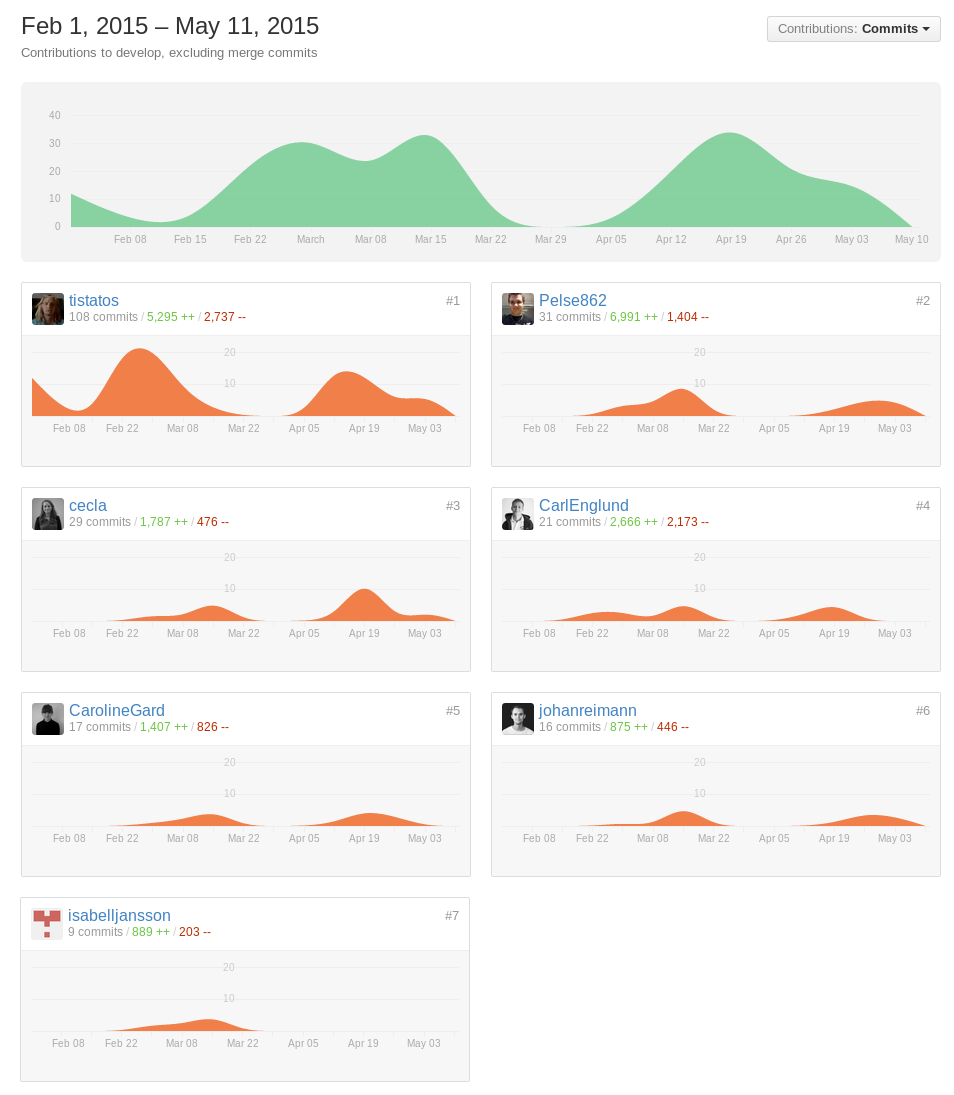
\includegraphics[scale=0.4]{bilder/gitstats.png}
  \label{fig:gitstats}
\end{figure}

\newpage
\chapter{Gantt schema}\label{app:gantt}
\begin{figure}[h]
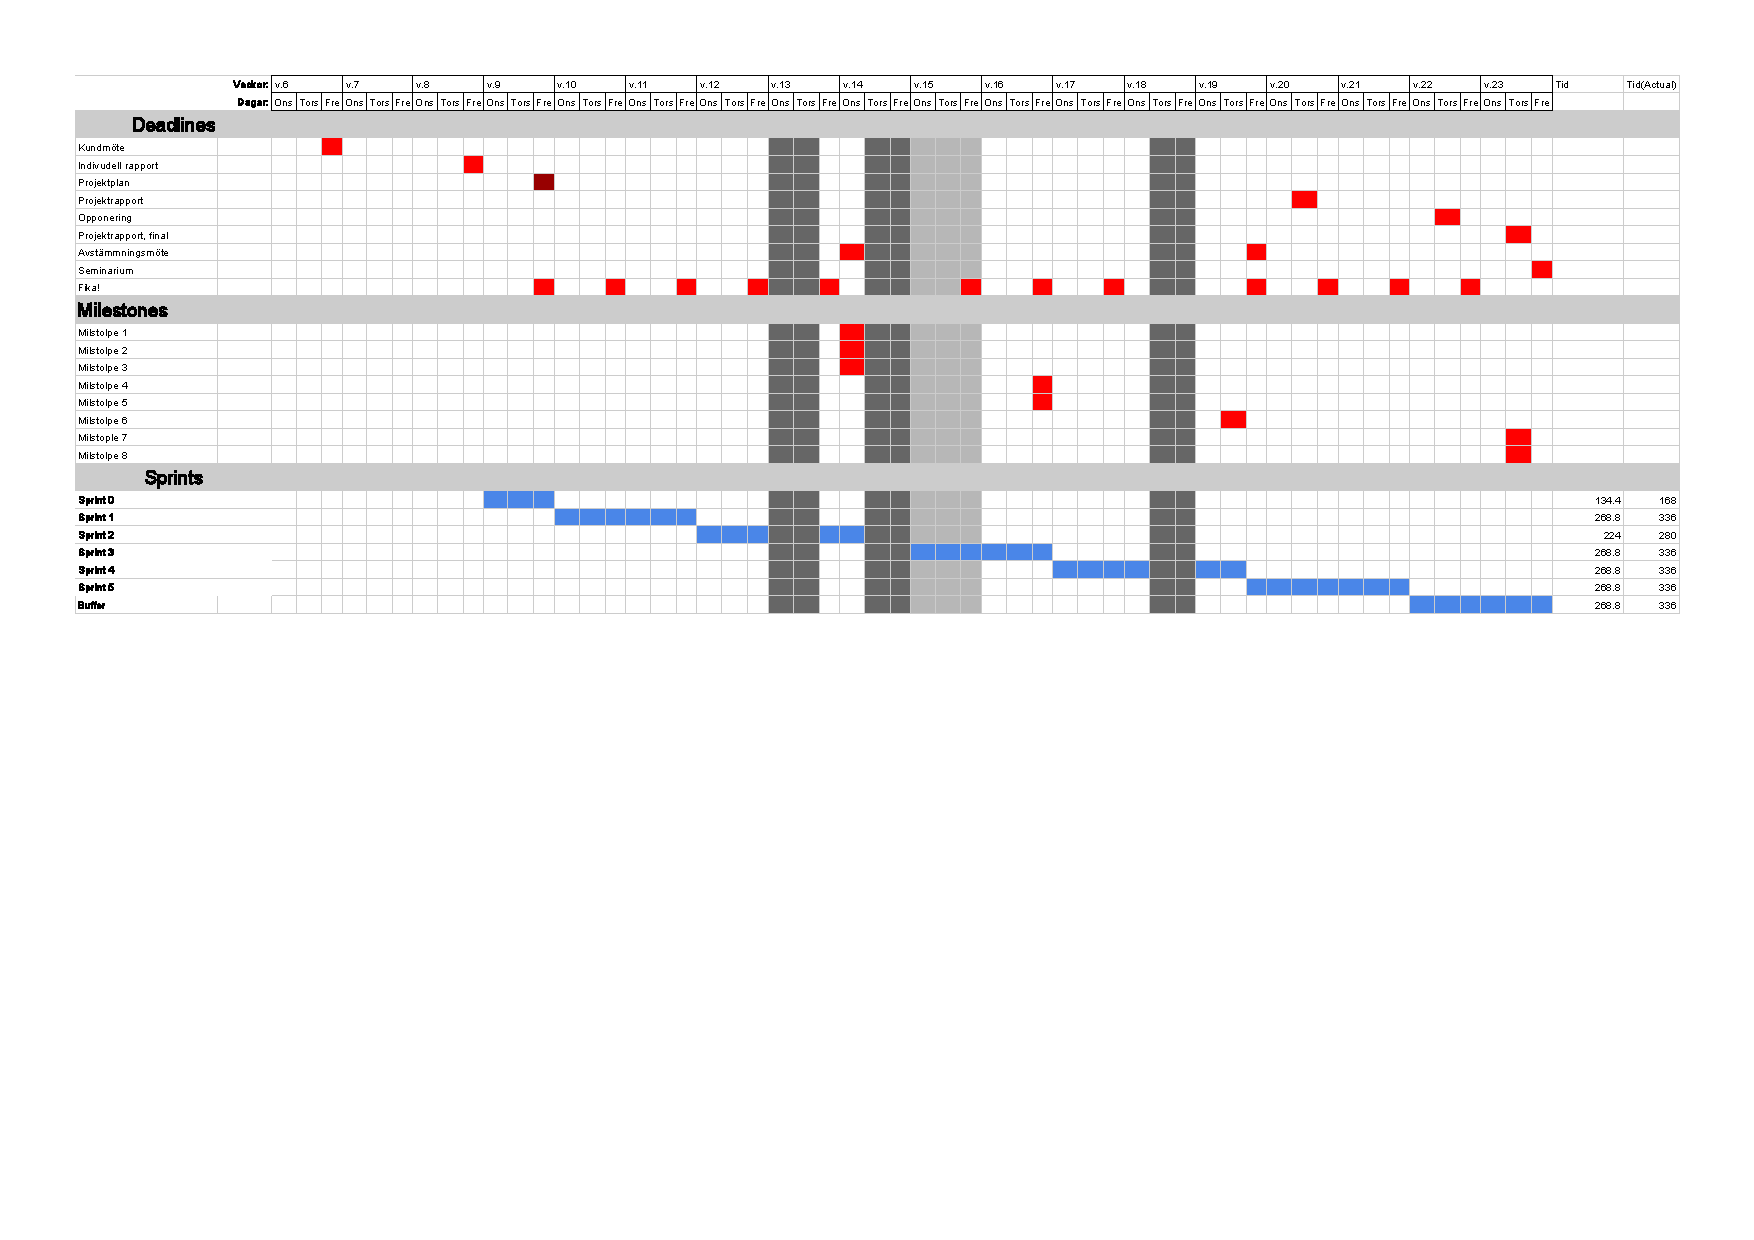
\includegraphics[angle=270,origin=c,scale=0.62]{Ganttschema.pdf}
\end{figure}

\end{document}
